%--------------------
% Packages
% -------------------
\documentclass[11pt,a4paper]{article}
\usepackage[utf8x]{inputenc}
\usepackage[T1]{fontenc}
\usepackage{mathptmx} % Use Times Font
\usepackage{float}
\usepackage{pdfpages}
\usepackage[pdftex]{graphicx} % Required for including pictures
\graphicspath{{figures/}}
\usepackage[pdftex,linkcolor=black,pdfborder={0 0 0}]{hyperref} %
% Format links for pdf
\usepackage{calc} % To reset the counter in the document after title page
\usepackage{enumitem} % Includes lists
\setitemize{noitemsep, topsep=0pt, partopsep=0pt, parsep=0pt}
\setenumerate{noitemsep, topsep=0pt, partopsep=0pt, parsep=0pt}
\frenchspacing % No double spacing between sentences
\usepackage[a4paper, lmargin=0.1666\paperwidth,
  rmargin=0.1666\paperwidth, tmargin=0.1111\paperheight,
bmargin=0.1111\paperheight]{geometry} %margins

% \usepackage[all]{nowidow} % Tries to remove widows
\usepackage[protrusion=true,expansion=true]{microtype} % Improves
% typography, load after fontpackage is selected

%-----------------------
% Set pdf information and add title, fill in the fields

%-----------------------
\hypersetup{
  pdfsubject = {},
  pdftitle = {Hands4Hire},
  pdfauthor = {Marta Borek \and Krzysztof Fijałkowski \and Tomasz
    Owienko \and Michał Jakomulski \and Wojciech Sekuła \and Arkadiusz
  Niedzielski}
}

% --------------------------
% Custom titlepage
% --------------------------
\makeatletter
\def\@maketitle{%
  \begin{center}
    
\includegraphics[width=0.3\textwidth]{logo.png}\par\vspace{1cm} % <- Path to your logo
    {\LARGE \@title \par}
    \vskip 1em
    {\large
      \lineskip .5em
      \begin{tabular}[t]{c}
        \@author
      \end{tabular}\par}
    \vskip 1em
    {\large \@date}
  \end{center}
}
\makeatother

\title{Hands4Hire - platform for connecting handymen with customers}
\author{Marta Borek \and Krzysztof Fijałkowski \and Tomasz Owienko
\and Michał Jakomulski \and Wojciech Sekuła \and Arkadiusz Niedzielski}
\date{}
%-----------------------
% Begin document
%-----------------------
\begin{document}

% \title{Hands4Hire - platform for connecting handymen with customers}
% \author{Marta Borek \and Krzysztof Fijałkowski \and Tomasz Owienko
% \and Michał Jakomulski \and Wojciech Sekuła \and Arkadiusz Niedzielski}
% \date{}

\maketitle

\setcounter{tocdepth}{2}
\tableofcontents
\newpage

\section{Introduction}
\textbf{Connecting Customers with Trusted Service Providers --- Simplified} \\

Traditionally, finding a trustworthy handyman or home repair specialist has relied heavily on word-of-mouth recommendations from friends or neighbors. While personal referrals can be valuable, this informal system often makes it difficult for customers to discover available professionals — especially on short notice — and for skilled service providers to consistently find work or expand their client base.

Our platform was designed to address these challenges by offering a centralized, transparent, and reliable digital solution for household services. Whether it’s plumbing, electrical repairs, or general handyman tasks, we simplify how Customers connect with Vendors based on availability, location, and service type.

At the same time, Vendors benefit from a dedicated space to showcase their services, manage scheduled visits, communicate with clients, and receive payments — all in one interface.

By streamlining this process, we aim to create a modern, scalable, and accessible ecosystem that benefits both sides of the marketplace.

\section{Requirements}

\subsection{Use cases}

\subsubsection{Create Profile}

\textbf{Actor:} Unregistered User

\noindent \textbf{Preconditions:} User is not yet registered or logged in

\noindent \textbf{Basic steps:}
\begin{enumerate}[noitemsep]
  \item User opens registration page
  \item Authenticates Google account
  \item Picks role
    \begin{itemize}[noitemsep]
      \item \textit{Vendor} - service provider
      \item \textit{Customer} - service recipient
    \end{itemize}
  \item Provides detailed data necessary for the role
  \item Pays registration fee
  \item System creates profile and redirects to dashboard
\end{enumerate}

\noindent \textbf{Postconditions:} Customer profile is stored in the system

\subsubsection{Edit Profile}

\textbf{Actor:} Registered Customer or Vendor

\noindent \textbf{Preconditions:} User is logged in

\noindent \textbf{Basic steps:}
\begin{enumerate}
  \item User navigates to ``Edit Profile'' from the home page
  \item Updates fields (e.g. skills, address, contact info)
  \item Submits changes
  \item System syncs data and confirms updates
\end{enumerate}

\noindent \textbf{Postconditions:} Profile gets updated and reflects latest data

\subsubsection{Update Calendar}

\textbf{Actor:} Registered Vendor

\noindent \textbf{Preconditions:} Vendor is logged in

\noindent \textbf{Basic steps:}
\begin{enumerate}
  \item Vendor opens calendar from profile page
  \item Adds/deletes available slots
  \item Can change status of a previously \textit{accepted} booking
    to \textit{canceled}
  \item Submits changes
  \item System syncs data and confirms updates
\end{enumerate}

\noindent \textbf{Postconditions:}
\begin{itemize}
  \item \textit{Canceled} booking removed from the calendar, still
    visible in history
  \item Updated calendar is reflected in searches and Vendor profile
  \item Customer gets notification about Booking's status change
\end{itemize}

\subsubsection{Search for Vendor}

\textbf{Actor:} Registered Customer

\noindent \textbf{Preconditions:} Customer is logged in

\noindent \textbf{Basic steps:}
\begin{enumerate}
  \item Customer opens search page
  \item Selects filters (e.g. type of service, geographical range,
    availability, customer rating)
  \item Submits search
  \item System displays matching Vendors profiles
\end{enumerate}

\noindent \textbf{Postconditions:} Filtered list is shown

\subsubsection{View Vendor Profile}

\textbf{Actor:} Registered Customer or Vendor

\noindent \textbf{Preconditions:}
\begin{enumerate}
  \item User is logged in
  \item Vendor Search/Filtering results available
  \item \textbf{Or For Customer:} Vendor already in Customer's Booking History
\end{enumerate}

\noindent \textbf{Basic steps:}
\begin{enumerate}
  \item Select Vendor from Search List or Booking History
  \item View Full Profile
    \begin{itemize}
      \item Contact Info
      \item Skills \& Experience
      \item Calendar availability
      \item User rating and comments from previous jobs
    \end{itemize}
\end{enumerate}

\noindent \textbf{Postconditions:} System displays public Vendor's Profile

\subsubsection{Book Vendor}

\textbf{Actor:} Registered Customer

\noindent \textbf{Preconditions:}
\begin{enumerate}
  \item Customer is logged in
  \item Selected Vendor's Profile open
\end{enumerate}

\noindent \textbf{Basic steps:}
\begin{enumerate}
  \item Select time slot from Vendor's Calendar
  \item Leave optional service note
  \item Submit request
\end{enumerate}

\noindent \textbf{Postconditions:}
\begin{itemize}
  \item Booking request stored in the system with \textit{pending} status
  \item Request added to Customer's booking history, visible in
    Customer's dashboard
  \item Notification sent to Vendor, request visible in Vendor's dashboard
\end{itemize}


\subsubsection{Identity Verification during Visit}

\textbf{Actor:} Registered Customer and Registered Vendor

\noindent \textbf{Preconditions:}
\begin{enumerate}
  \item Customer is logged in
  \item Vendor is logged in
  \item Current time corresponds to predefined range before/during/after the scheduled Booking time (e.g., Booking time slot + 30 minutes before and after the slot )
\end{enumerate}

\noindent \textbf{Basic steps:}
\begin{enumerate}
  \item Customer gets notification about the upcoming visit + verification code (both email and in-app)
  \item Vendor selects appropriate Booking from their Booking List
  \item Selects ``Verify''
  \item Enters Customer's code into a form
  \item Vendor sends completed form
  \item Vendor gets immediate feedback on whether the code matches \& option to retry if incorrect
\end{enumerate}

\noindent \textbf{Postconditions:}
\begin{itemize}
  \item Booking gets status update to \textit{verified} in Customer's and Vendor's Booking Histories
  \item Notification about the Booking verification sent to both parties
\end{itemize}

\subsubsection{View Customer Profile}

\textbf{Actor:} Registered Vendor or Customer

\noindent \textbf{Preconditions:}
\begin{enumerate}
  \item User is logged in
  \item Vendor received Booking from a Customer
  \item OR User views comments left by other Customers on Vendor's Profile
\end{enumerate}

\noindent \textbf{Basic steps:}
\begin{enumerate}
  \item Select Customer from Booking request, or Comments List
  \item View Full Profile
    \begin{itemize}
      \item Contact Info
      \item Booking History
      \item Comments and ratings for previous jobs
    \end{itemize}
\end{enumerate}

\noindent \textbf{Postconditions:} System displays public Customer Profile

\subsubsection{Accept or Decline Booking}

\textbf{Actor:} Registered Vendor

\noindent \textbf{Preconditions:}
\begin{enumerate}
  \item Vendor received Booking from a Customer
  \item Booking status is \textit{pending}
\end{enumerate}

\noindent \textbf{Basic steps:}
\begin{enumerate}
  \item Vendor received a Booking Request notification (in-app/e-mail)
  \item Notification redirection to Booking Request, with eventual
    authentication step
  \item OR Open Booking request directly from dashboard
  \item Booking Request shows:
    \begin{itemize}
      \item Customer who placed the request
      \item Date, Time \& Duration
      \item Service note from the Customer
      \item Current status \textit{pending, canceled}
    \end{itemize}
  \item If not \textit{canceled} Vendor can Accept or Decline with
    designated buttons
  \item System confirms the status update
\end{enumerate}

\noindent \textbf{Postconditions:}
\begin{itemize}
  \item Booking status changes to \textit{accepted} or \textit{declined}
  \item If \textit{accepted}, is now visible in the Vendor
    availability Calendar and will be reflected in the Vendor Searches
  \item Customer gets a notification about the Booking status change
\end{itemize}

\subsubsection{View \& Cancel Booking Status}

\textbf{Actor:} Registered Customer

\noindent \textbf{Preconditions:}
\begin{enumerate}
  \item Customer placed at least one Booking
\end{enumerate}

\noindent \textbf{Basic steps:}
\begin{enumerate}
  \item Customer goes to Booking History on home page
  \item Selects an entry to open a Booking page
  \item OR Notification about Booking status update redirection to
    Booking Request, with eventual authentication step
  \item Booking entry shows:
    \begin{itemize}
      \item Booked Vendor
      \item Date, Time \& Duration
      \item Service note from the Customer
      \item Current status \textit{accepted, declined, pending, canceled}
    \end{itemize}
  \item If \textit{accepted} or \textit{pending}, Customer can cancel
    the request
  \item System confirms eventual status update
\end{enumerate}

\noindent \textbf{Postconditions:}
\begin{itemize}
  \item Booking status changes to \textit{canceled}
  \item If previously \textit{accepted} by Vendor, it is now
    removed from the Vendor availability Calendar and will be
    reflected in the Vendor Searches
  \item Vendor gets a notification about the Booking status change
\end{itemize}

\subsubsection{Contact Between Customer \& Vendor}

\textbf{Actor:} Registered Customer or Vendor

\noindent \textbf{Preconditions:}
\begin{enumerate}
  \item Booking request placed by Customer
  \item OR User Profile viewed
  \item OR Previously registered in the chat history
\end{enumerate}

\noindent \textbf{Basic steps:}
\begin{enumerate}
  \item User selects ``Message'' for a new chat from Recipient's Profile
  \item OR an active chat from chats list on the dashboard
  \item Enters message in chat interface
  \item Sends message
  \item Recipient receives notification
\end{enumerate}

\noindent \textbf{Postconditions:}
\begin{itemize}
  \item Notification about a new message sent to the Recipient
  \item System stores new message and updates the chat history
  \item If no previous chat history with the Recipient, System adds
    new chat to the chat history, available from User dashboard
\end{itemize}

\subsubsection{Comment \& Rate Past Booking }

\textbf{Actor:} Registered Customer

\noindent \textbf{Preconditions:}
\begin{enumerate}
  \item Booking accepted by Vendor
  \item Successful identity verification of Booking parties
  \item Booking time slot passed
\end{enumerate}

\noindent \textbf{Basic steps:}
\begin{enumerate}
  \item User selects Booking from their Booking History
  \item User selects ``Rate and Comment''
  \item Enters rating within a specified range
  \item AND/OR Writes a comment  
  \item Selects ``Publish''
\end{enumerate}

\noindent \textbf{Postconditions:}
\begin{itemize}
  \item Notification about a new rating sent to the Vendor
  \item System stores new rating and updates the affected Vendor's profile
  \item Booking marked with \textit{rated} status in Client's Booking History
  \item Client cannot leave another comment/rating on that Booking
\end{itemize}

\subsection{Functional requirements}

\subsubsection{User Profile Management}

\paragraph{Registration}

\begin{itemize}
  \item Through Google account
  \item Requires a one time registration fee
\end{itemize}

\paragraph{User Profile}
\begin{itemize}
  \item Each user owns a profile with editable personal data
  \item Additionally:
    \begin{itemize}
      \item \textit{Vendors} profiles contain:
        \begin{itemize}
          \item skills and specialization areas
          \item User ratings and comments from previous jobs
          \item Calendar with availability
        \end{itemize}
      \item \textit{Customers} profiles contain:
        \begin{itemize}
          \item Booking history
          \item Ratings for previous bookings
        \end{itemize}
    \end{itemize}
\end{itemize}

\paragraph{Ratings and Comments}
\begin{itemize}
  \item Customers can leave feedback for the jobs from the Booking History
  \item Feedback in a form of a star range rating (scale up to 5 or
    10) and an optional comment
\end{itemize}

\subsubsection{Calendar}
\begin{itemize}
  \item Vendors manage their availability in a personal calendar,
    which is visible on their profile
  \item Customers view Vendors's calendar on their profile and can
    make booking requests within the free slots
\end{itemize}

\subsubsection{Bookings Management}

\paragraph{Vendor Search}

System for searching and filtering Vendors profiles according to:
\begin{itemize}
  \item skills
  \item price
  \item location or geographical range
  \item availability
  \item customer rating
\end{itemize}

\paragraph{Booking placement}

Through calendars available at Vendor profiles, Customers can place bookings:
\begin{itemize}
  \item Bookings can be accepted or declined by Vendors
  \item Bookings can be canceled by both Vendors and Customers,
    regardless of their status
  \item Status change of a Booking results in a notification to the second party
\end{itemize}

\paragraph{Report generation}

Automatic statistical report generation per Vendor profile. Includes:
\begin{itemize}
  \item bookings count
  \item work hours
  \item earnings
  \item types of services
\end{itemize}

\subsubsection{Communicator}
\begin{itemize}
  \item User Chat for communication between Vendors and Customers
  \item Code for Booking confirmation and identity authentication sent via chat
\end{itemize}

\subsection{Non-functional requirements}
\begin{itemize}
\item \textbf{Architecture}
  As dictated by the general project requirements:
  \begin{itemize}
  \item Application is hosted on a public cloud (Google Cloud Provider)
  \item Application consists of at least 3 types of microservices
  \item The infrastructure build and setup are automated with the use of automation tool, Terraform
  \item Database and state are owned by each microservice type separately, with two of them having private cache of the other's data subset
  \end{itemize}
\item \textbf{Performance \& Responsiveness}
  System should support real-time updates for chat and booking confirmations.
\item \textbf{Authorization \& Security}
  \begin{itemize}
  \item User identity verification is done with the use of trusted identity provider Google OAuth 2.0
  \item Authentication in payment processing is done via Stripe secret keys, securely stored in GCP Secret Manager
  \end{itemize}
\item \textbf{Maintainability \& Observability}
  \begin{itemize}
  \item The use of automation tool, Terraform, allows for reproducible deployment
  \item All microservices emit structured messages to Kafka and the Google Cloud Logging Agent
  \end{itemize}
\end{itemize}

\section{System Architecture}

\subsection{Visit Scheduler Module}

\subsection{Visit Manager Module}

\subsubsection{Routing}
\begin{itemize}
\item \textbf{\slash register} - submit User's registration details
\item \textbf{\slash register\_visit} - visit registration, passed from the Visit Scheduler module, which handles Customer's input
\item \textbf{\slash client/my\_visits} - 
\item \textbf{\slash vendor/my\_visits} - returns a list of visits that a Vendor has scheduled
\item \textbf{\slash get\_visit\_code} - returns generated code for Vendor's identity confirmation during the visit (hash of visit\_id for simplicity reasons)
\item \textbf{\slash check\_visit\_code} - returns information about validity of the code submitted in a request by the Customer
\item \textbf{\slash add\_opinion} - enabled only after the scheduled visit took place, allows Customer to leave a rating (1-5 scale) and review
\end{itemize}


\subsection{User Chat}

\subsection{Web Server}

\subsection{Kafka}

\begin{figure}[H]
  \centering
  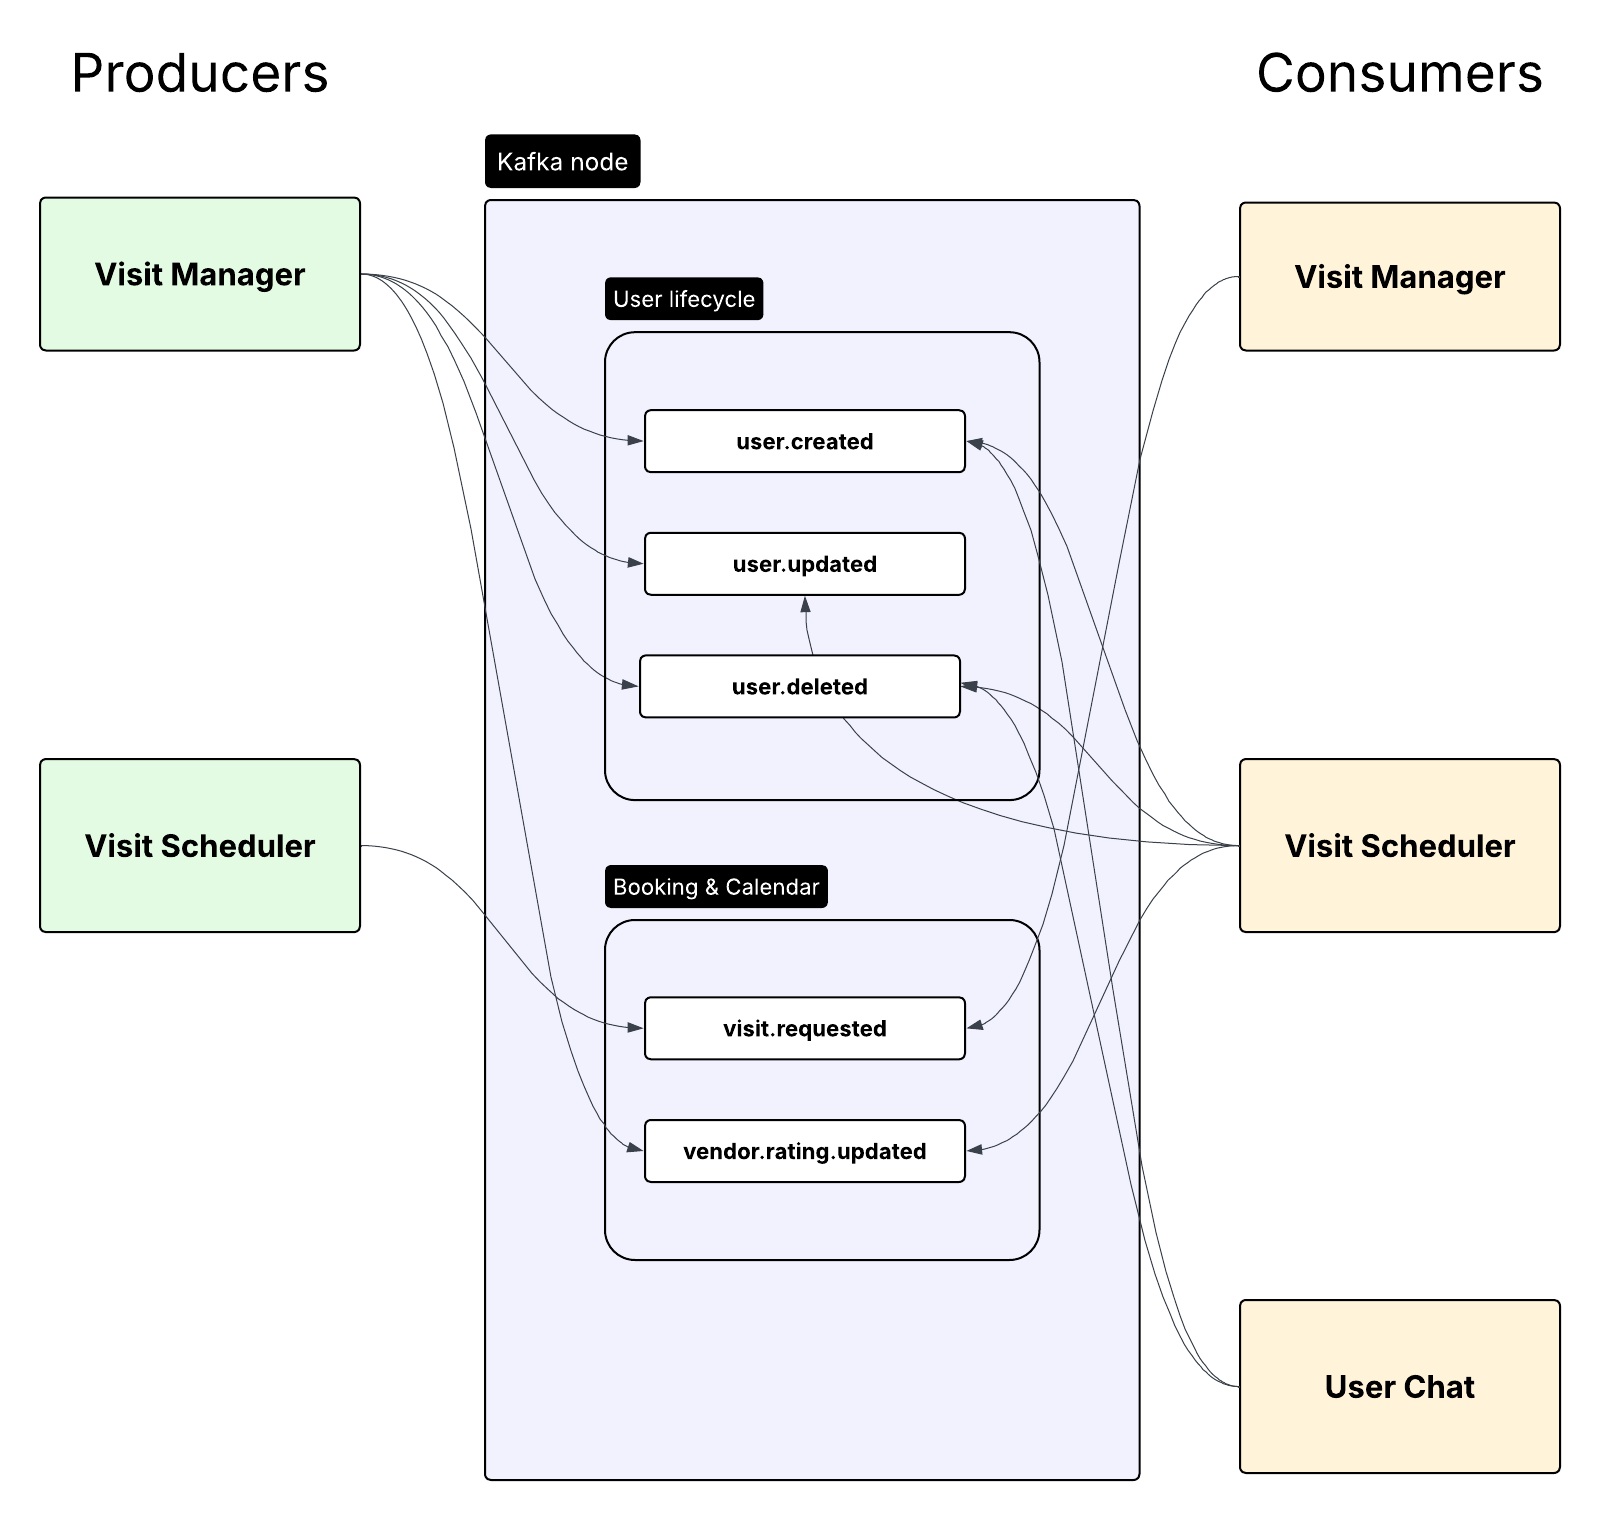
\includegraphics[width=\textwidth]{H4H_Kafka.png}
  \caption{Kafka Topics Diagram}
  \label{fig:kafka-topics-diagram}
\end{figure}

\section{Security threat model}

\begin{figure}[H]
  \centering
  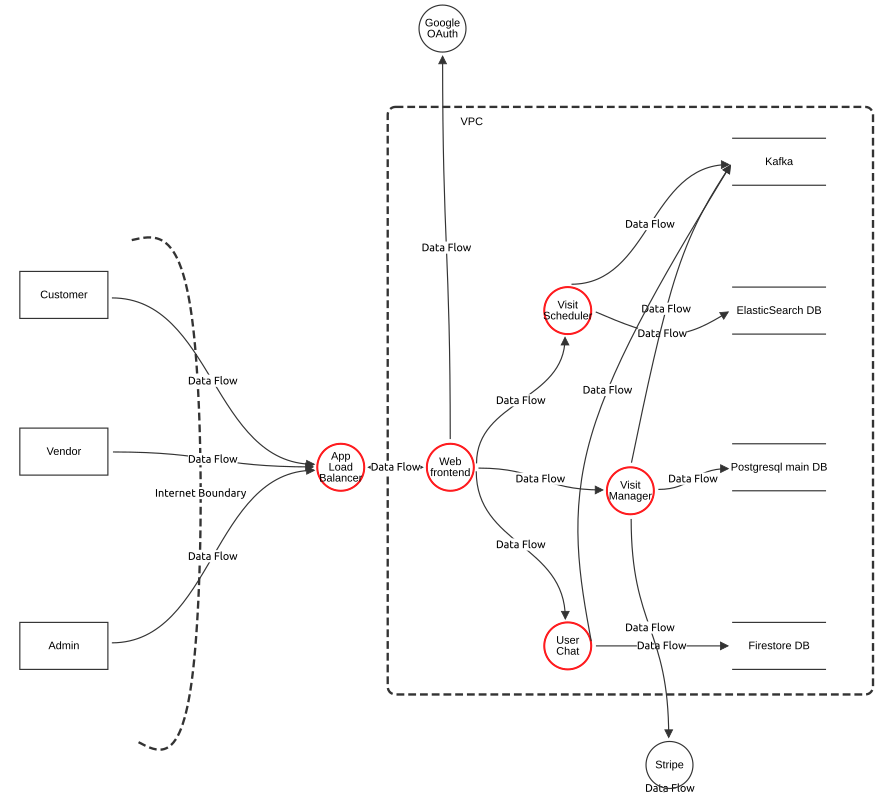
\includegraphics[width=\textwidth]{DFD-threat-model.png}
  \caption{Threat modeling Data Flow Diagram}
  \label{fig:DFD-threat-model}
\end{figure}


\includepdf[pages=-]{figures/H4H-threat-report.pdf}
\end{document}
